\chapter{Implementation}
\label{chapter:implementation}
\section{Option Pricing}
\label{section:Option Pricing}
The theoretical models presented in Chapter \ref{chapter:background} attempt to replicate the movements of real-world stock prices. With these predictions, we should be able to better reproduce real option prices than if we assumed a simple constant volatility, like Black \textit{et al.}

Currently, the two most used methods to computationally price options are known as \emph{finite differences}~\cite{Hull} and \emph{Monte Carlo}~\cite{Glasserman}.

The finite differences method is an extremely fast procedure when used to price either European or American-type options, making it very appealing in these circumstances. However, when applied to other option types whose value depends on the stock prices until maturity (e.g. Asian options), the algorithm becomes very slow, rendering it almost useless.
The implementation of both Heston and SABR models (presented before) using finite differences can be found in deGraaf~\cite{deGraaf}.


With the Monte Carlo algorithm, we begin by simulating a very large number of stock price paths (e.g. 100,000 simulations). The option's payoff is then calculated for each of these simulated paths and averaged, providing a fairly good estimate of the option's value. This algorithm can be easily adapted to price exotic options, making it very attractive in such cases.
In the past, simulating all the stock price paths took prohibitively long computation times and this method was often discarded for this reason. However, with the recent advancements in computer hardware and new algorithmic developments, such as GPU implementation, this shortcoming has been, to some extent, solved, making the Monte Carlo algorithm quite popular in the present.
For these reasons, the Monte Carlo method will be used for the analysis of the models introduced in Chapter \ref{chapter:background}.


\subsection{Simulating stock prices}
\label{subsection:Simulating stock prices}
As stated, to implement the Monte Carlo algorithm, one needs to simulate stock price paths. However, by analyzing eq.\eqref{GBM}, we can see that the stock prices depend on a Brownian motion process which, due to its self-similarity, is not differentiable~\cite{Mikosch}. It follows that stock price paths can never be exactly simulated. Despite this, we can approximate the movement of stock price paths by discretizing the Brownian motion process in time, thus solving its self-similarity problem. Two of the most common discretization procedures are presented below.

\subsubsection{Euler–Maruyama discretization}
\hl{put this in background section?}

One of the simplest and most used discretization methods is known as \emph{Euler–Maruyama discretization}, and can be applied to stochastic differential equations of the type
\begin{equation}\label{SDE}
dX(t)=a(X(t))dt+b(X(t))dW(t),
\end{equation}
\noindent where $a(X(t))$ and $b(X(t))$ are some given functions of $X(t)$ and $\{W(t),\ t>0\}$ defines a one-dimensional Brownian motion process.
To apply this discretization, we begin by partitioning the time interval $[0,T]$ into $N$ subintervals of width $\Delta t=T/N$ and then iteratively define
\begin{equation}
X_{n+1}=X_n+a(X_n)\Delta t+b(X_n)\Delta W_n,\ \ \ n=1,\ldots,N
\end{equation}
\noindent where $\Delta W_n=W_{t+\Delta t}-W_{t}$.
Using the known properties of Brownian motion processes, it can be shown that $\Delta W_n\sim \sqrt{\Delta t}Z$, where $Z\sim N(0,1)$ defines a standard normal distribution.

Applying this discretization to the Geometric Brownian motion followed by stock price paths, as seen in eq.\eqref{GBM}, we arrive at
\begin{equation}
S(t+\Delta t)=S(t)+rS(t)\Delta t+\sigma(S(t),t)S(t)\sqrt{\Delta t}Z.
\end{equation}

Due to its simplicity, the Euler–Maruyama discretization method is the most common in the simulation of stock price paths whenever we have constant or deterministic volatilities.


\subsubsection{Milstein Discretization}
For stochastic volatility models, such as Heston and SABR, where the volatility itself follows a stochastic differential equation, the Euler–Maruyama discretization may not be sufficiently accurate. In these cases, we can apply the more precise Milstein method~\cite{Milstein}, defined as
\begin{equation}
X_{n+1}=X_n+a(X_n)\Delta t+b(X_n)\Delta W_n+\frac{1}{2}b(X_n)b'(X_n)((\Delta W_n)^2-\Delta t),
\end{equation}
\noindent where $b'(X_n)$ denotes the derivative of $b(X_n)$ w.r.t. $X_n$. Note that when $b'(X_n)=0$, the Milstein method degenerates to the simpler Euler–Maruyama discretization.

Applying this discretization to the Heston model, we arrive at
\begin{equation}
S(t+\Delta t)=S(t)+rS(t)\Delta t+S(t)\sqrt{\nu(t)}\sqrt{\Delta t}Z_1+\frac{1}{2}\nu(t)S(t)\Delta t(Z_1^2-1),
\end{equation}
\begin{equation}
\nu(t+\Delta t)=\nu(t)+\kappa(\overline{\nu}-\nu(t))\Delta t+\eta\sqrt{\nu(t)\Delta t}Z_2+\frac{\eta^2}{4}\Delta t(Z_2^2-1),
\end{equation}
\noindent where $Z_1$ and $Z_2$ are two normal random variables with a correlation of $\rho$.


Applying the Milstein discretization to the SABR model results in
\begin{equation}
\begin{split}
S(t+\Delta t)=&S(t)+rS(t)\Delta t+e^{-r(T-t)(1-\beta)}\sigma(t)S^\beta(t)\sqrt{\Delta t}Z_1+\\
&+\frac{\beta}{2}e^{-2r(T-t)(1-\beta)}\sigma^2(t)S^{2\beta-1}(t)\Delta t(Z_1^2-1),
\end{split}
\end{equation}
\begin{equation}
\sigma(t+\Delta t)=\sigma(t)+\nu\sigma(t)\sqrt{\Delta t}Z_2+\frac{\nu^2}{2}\sigma(t)\Delta t(Z_2^2-1),
\end{equation}
\noindent where again $Z_1$ and $Z_2$ are two normal random variables with a correlation of $\rho$.

In both models we need to generate the two correlated normal variables, $Z_1$ and $Z_2$, which we can produce from
\begin{equation}\label{normcorr}
\begin{split}
&Z_1\sim N(0,1);\\
&Z_2=\rho Z_1+\sqrt{1-\rho^2}Y,
\end{split}
\end{equation}
\noindent where $Y\sim N(0,1)$ is uncorrelated with $Z_1$.

Because it is more precise, the Milstein method will be used in the implementation of both Heston and SABR stochastic volatility models. The simpler Euler–Maruyama discretization will be assumed for both constant and Dupire's local volatility.


\subsection{Pricing options from simulations}
\hl{this should come before the discretization methods?}

To price options using the Monte Carlo algorithm, we generate $M$ paths by recursively calculating $\{S_i(t),\ \ i=1,\ldots,M\}$, using either of the discretization methods presented before.

When the stock price at the maturity, $S_i(T)$, is obtained for all paths, the option's payoff for each path is calculated from eq.\eqref{callput}. We then average all these results and discount them back to the present, obtaining the (call) option's value
\begin{equation}
C(K,T)=e^{-rT}\frac{1}{M}\sum_{i=1}^M\max\left(S_i(T)-K,0\right).
\end{equation}

It is important to note that, the smaller our subintervals $\Delta t$ are, the better is the approximation done when discretizing the Brownian motion process. However, by decreasing $\Delta t$ we increase the number of intervals and with it the number of calculations required to obtain each $S_i(T)$. The compromise between computation time and precision must be handled appropriately.
 \hl{put some image here to exemplify the different time steps dt}



\iffalse
depend on a Brownian motion process, it follows that it is not differentiable. For this reason, it's impossible to exactly simulate such a process. An approximation is possible, however, using discrete jumps of length $\Delta t$ and using the Brownian motion property $W(t)\sim \sqrt{t}N(0,1)$~\cite{Mikosch}, with $N(0,1)$ being a normal distribution with 0 expected value and 1 variance.
We can then simply discretize eq. \eqref{BS} into
\begin{equation}
S(t+\Delta t)=S(t)+rS(t)\Delta t+\sqrt{\Delta t}\sigma S(t)N(0,1),
\end{equation}
\noindent where $\Delta t$ corresponds to a given time step. An example of this discretization is illustrated in \autoref{fig:GBM} with the realization of three sample paths.

\begin{figure}[H]
    \centering
      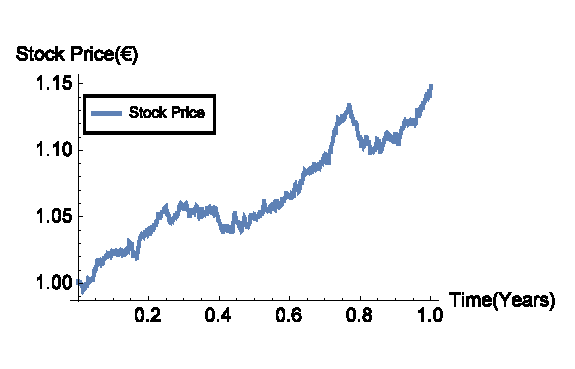
\includegraphics[width=0.9\columnwidth]{GBM.eps}
      \caption{Example of three GBM processes, using the parameters $r=\SI{0.06}{\per\year}$, $\sigma=0.05$, $S(0)=\SI{1}[\EUR]{}$ and time steps $\Delta t=10^{-3}\SI{}{\year}$.}\label{fig:GBM}
    \end{figure}
    
By simulating a large number of paths, some underlying tendencies might become apparent, which will prove useful in option pricing.


 American options, however, pose a much greater challenge.  Unlike European options, no analytic pricing model currently exists for this type of derivatives. Several numerical models have been proposed in the past in an attempt to solve this problem~\cite{Wilmott1,Hull}, such as the Longstaff-Schwartz algorithm~\citep{Longstaff}, which we shall approach in later sections of the present thesis.
\fi 

 
 
 
\section{Model Calibration}
\label{section:Model Calibration}
Both SABR and Heston stochastic volatility models contain variables that need to be calibrated in order to appropriately replicate market option prices.


Calibrating the models' parameters means finding the optimal values for these parameters such that the difference between the prices of real market options and options priced under the models' assumptions is minimized. This difference should be measured with a cost function such as
\begin{equation}\label{cost}
\mathrm{Cost}(\theta)=\sum_{i=1}^n\sum_{j=1}^m\left(\frac{C_{\mathrm{market}}(T_i,K_j)-C_{\mathrm{model}}(\theta;T_i,K_j)}{C_{\mathrm{market}}(T_i,K_j)}\right)^2,
\end{equation}
\noindent where we denote $\theta$ as the model's parameter set and $C_{\mathrm{model}}(\cdot)$ and $C_{\mathrm{market}}(\cdot)$ correspond to the model and market option prices, respectively, for maturities $T_i,(i=1,\ldots,n)$ and strikes $K_j,(j=1,\ldots,m)$.

\hl{or cost function using implied volatility:}
This difference should be measured with a cost function such as
\begin{equation}\label{cost}
\mathrm{Cost}(\theta)=\sum_{i=1}^n\sum_{j=1}^m\left(\frac{\sigma_{imp,\mathrm{mkt}}(T_i,K_j)-\sigma_{imp,\mathrm{mdl}}(\theta;T_i,K_j)}{\sigma_{imp,\mathrm{mkt}}(T_i,K_j)}\right)^2,
\end{equation}
\noindent where we denote $\theta$ as the model's parameter set and $\sigma_{imp,\mathrm{mkt}}(\cdot)$ and $\sigma_{imp,\mathrm{mdl}}(\cdot)$ correspond to the real-market and model implied volatilities, respectively, for maturities $T_i,(i=1,\ldots,n)$ and strikes $K_j,(j=1,\ldots,m)$.
\hl{why this cost function? higher weights on near-the-money options, is least squares,...}

To obtain the value of the cost function for a given set of parameters, we need to calculate $m\times n$ model option prices. We could achieve this by applying the Monte Carlo method along with the discretization procedures described before.
Because we want to calibrate the model's parameters, a large number of instances of the cost function will have to be executed for our optimization algorithms to converge to an optimal solution.
Thus, it can be seen that a very great number of Monte Carlo pricers will have to be executed. Even with GPU implementation and recent hardware, using Monte Carlo to calibrate the model's parameters will become prohibitively slow. We could reduce the computation time by limiting the number of simulated paths, but this would introduce a high amount of noise in the prices, making the optimization procedure nearly impossible.
Thus, we can conclude that though the Monte Carlo algorithm is very useful to price a small amount of options, it is nearly useless in the calibration procedures required to use both the Heston and SABR models.

\hl{replace "Monte Carlo" by "MC"?}

Fortunately, both Heston and SABR have closed-form solutions, shown in eqs. \eqref{CH}, \eqref{sabr} and \eqref{dynsabr}, that we can use to directly price the options with each model's parameters, without the need to run the slow Monte Carlo pricer. The optimization algorithms should then converge much faster to the optimal solution for the model's parameters. This characteristic of both models is indeed what makes them so appealing. 






\subsection{Optimization Algorithms}
There are several possible methods to find the parameter set that minimizes the cost function shown in eq.\eqref{cost} \hl{(if we use the implied vol cost, change reference)}.
Our main concern when choosing the best algorithms for calibration is the nonlinearity of the cost function. This is problematic because several local minima might exist and an unsuitable algorithm may get stuck in these points, causing the globally optimal solution to not be found.

With this issue in mind, we selected two powerful algorithms known as \emph{Multi-Start}~\cite{Ugray} and \emph{CMA-ES}~\cite{Hansen2} (short for Covariance Matrix Adaptation Evolution Strategy), which we will summarize below. It should be noted that we will only provide a general idea of how each optimizer works. For detailed descriptions, the original sources should be consulted.

\hl{how to deal with parameter boundaries? (All these algorithms enable the use of bounds which are required for our model parameters (e.g. the correlation parameter, $\rho$, in both Heston and SABR is obviously contained between $-1$ and $1$). Furthermore, they all require an initial guess at the values of the parameters, $\theta_0$, from which they will try to converge.)}

The optimization algorithms will search the $D$-dimensional sample space ($D$ corresponds to the number of parameters of each model), for the optimal solution. Each point in this space corresponds to a possible set of parameters, $\theta$.

\subsubsection{Multi-Start Optimizer}
The Multi-Start optimizer is nothing more than the application of a simple optimization algorithm with multiple starting conditions.


This algorithm starts by generating a set of $N$ different starting points, $\theta_{0,i},\ \ i=1,\ldots,N$, distributed in the sample space. These can be generated at random (i.e. by sampling from a uniform distribution) or using some complex meta-heuristic such as scatter search~\cite{Ugray}. For simplicity, and because it is usually faster to execute, we will use randomized sampling.


The procedure then applies a weak optimizer to each of these starting points, finding one (local) minimum for all of them. Examples of such simple optimizers are the \emph{Active Set Method}, \emph{Sequential Quadratic Programming}, among others. These optimizers are weak because they are only expected to converge to the (local) optimum closest to their starting point. They are, however, very fast to converge.

After a local minimum is found for each of the selected starting points, the minimum where the cost function is minimized is chosen as optimal solution.

This procedure is depicted in Algorithm \ref{MSOpt}.

\begin{algorithm}[H]\label{MSOpt}
\DontPrintSemicolon
Generate $\theta_{0,i},\ \ i=1,\ldots,N$\tcc*[r]{Multiple starting points}
 \For{$i=1,\ldots,N$}{
  Run weak optimization algorithm with starting point $\theta_{0,i}$\;
  Calculate $\mathrm{Cost}(\theta_i')$ for the minimum found, $\theta_i'$\;
 }
 Optimal parameters: $\theta^{*}=\underset{\theta_i'}{\arg\min}\left\{\mathrm{Cost}(\theta_i')\right\}$\;
 \caption{Multi-Start Optimizer}
\end{algorithm}
\ 

One of the advantages of the Multi-Start is the fact that, because the weak algorithms are independent of one another (assuming no meta-heuristics are used), we can run them in parallel, further increasing calibration speed.
As a disadvantage, we can point out the fact that, for highly nonlinear functions, a large number of starting points may be required, decreasing the calibration speed.

As a sidenote, we should point out that, for a large enough starting sample set, $N$, the global minimum will be found with probability 1, even for highly nonlinear objective functions. Though the proof is trivial, this remark is important, because we need a compromise between a large starting set that will take too long to compute and a small data set that might return a non-optimal result.


This optimizer is implemented in MATLAB with the \emph{MultiStart} function~\cite{MATLABMS}

\subsubsection{CMA-ES Optimizer}
The CMA-ES optimizer belongs to the class of evolutionary algorithms. These methods are based on the principle of biological evolution: at each iteration (generation), new candidate solutions (individuals) are generated from a given random distribution (mutation) obtained using the data (genes) of the previous solutions (parents). Of these newly generated solutions (individuals), we select the ones where the cost function is minimized (with the best fitness) to generate the candidate solutions of the next iterations (to become the parents of the next generation) and reject the others.



As for the CMA-ES in particular, the algorithm takes $\lambda$ samples from a multivariate normal distribution in the $D$-dimensional sample space
\begin{equation}
N(\mathbf{x;m,C})=\frac{1}{\sqrt{(2\pi)^D|\mathrm{det}\mathbf{C}|}}\mathrm{exp}\left(-\frac{1}{2}(\mathbf{x}-\mathbf{m})^T\mathbf{C}^{-1}(\mathbf{x}-\mathbf{m})\right),
\end{equation}
\noindent where $\mathbf{m}$ and $\mathbf{C}$ correspond to the distribution's mean vector and covariance matrix.
These $\lambda$ samples are our candidate solutions.

We classify each of these points according to their fitness (i.e. the cost function's value for a given point). We then select the $\mu$ samples with the lowest cost and discard the others. These new points will be the parents of the next generation.

The number of candidate solutions generated at each step, $\lambda$, and the ones that remain after classification, $\mu$, can be chosen arbitrarily, but an adequate heuristic is to choose $\lambda=\left\lfloor4+3\log D\right\rfloor+1$ and $\mu=\left\lfloor\lambda/2\right\rfloor+1$.

With these $\mu$ points, we generate a new mean and covariance matrix for the multivariate normal distribution.
At each iteration, the new mean is produced from a weighted average of the points, with the weights proportional to each point's fitness.
The method for the covariance matrix update is rather complex and depends not only on the $\mu$ best samples but also on the values of previous covariance matrices. All the basic equations required for the implementation of this optimizer can be found in Appendix \ref{chapter:CMAESAlg}. For a more detailed explanation, as well as other aspects of the algorithm, see Hansen \cite{Hansen}.

These sampling-classification-adaptation steps are repeated until a some stopping criterion is met. Examples of stopping criteria include a fixed number of iterations or an error threshold.

\hl{mean vector m gets closer and closer to the global optimum at each iteration}

This procedure is summarized in Algorithm \ref{CMAES}.

\begin{algorithm}[H]\label{CMAES}
\DontPrintSemicolon
Define mean vector $\mathbf{m}=\theta_0$\tcc*[r]{Initial guess}
Define covariance matrix $\mathbf{C}=I$\;
\While{Termination criterion not met}{
  Sample $\lambda$ points from multivariate normal distribution $N(\mathbf{x;m,C})$\;
  Calculate the cost for all generated points and keep the $\mu$ best. Discard the rest\;
  Update the mean vector and covariance matrix (using eqs.\eqref{mean} and \eqref{covariance})\;
 }
 Optimal parameters: $\theta^{*}=\mathbf{m}$\;
 \caption{CMA-ES Optimizer}
\end{algorithm}
\

The complexity of the covariance matrix adaptation process makes CMA-ES a very robust optimization algorithm, enabling it to find the global optimum of highly nonlinear functions~\cite{DilaoCMA}.
Furthermore, the CMA-ES is almost parameter free. It simply requires an initial guess, to generate the starting mean vector, and the algorithm should converge.
As for disadvantages, there may be cases where the convergence of this algorithm is slow, and the Multi-Start may be used as an alternative when a fast convergence is required, though the CMA-ES will outperform the Multi-Start algorithm in terms of precision.

This optimizer was implemented by Hansen in MATLAB (as well as in other computer languages) as function \emph{purecmaes}~\cite{CMAES}.



\hl{CMA-ES seems to outperform Multi-Start whenever the number of dimensions increases}

